% @Author: AnthonyKenny98
% @Date:   2020-03-19 12:56:13
% @Last Modified by:   AnthonyKenny98
% @Last Modified time: 2020-04-05 16:37:50

\section{Justification of Modelling UAV as Prism}
\label{section:rrt_appendix_modelling}
    While it is possible for a \gls{UAV} to be modelled in precise detail, taking into account its exact shape, more often \glspl{UAV} are modelled as a 3D prism in motion planning problems, for the following reasons:
    \begin{itemize}
    \item It is a rare case that the negative space gained by modelling in such detail is utilised
    \item Representation of drone's configuration is much more complex.
    \item Computing edge collisions is much more computationally intensive.
    \end{itemize}

    % @Author: AnthonyKenny98
% @Date:   2020-04-05 12:55:29
% @Last Modified by:   AnthonyKenny98
% @Last Modified time: 2020-04-05 15:43:13

\begin{figure}[H]
\begin{centering}

\begin{tabular}{cc}
\begin{subfigure}{0.45\linewidth}
    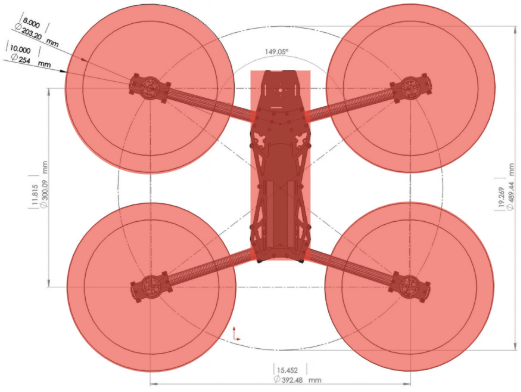
\includegraphics[width=\linewidth]{appendices/rrt/img/DroneNegSpace.png}
    \caption{}
    \label{subfig:dronenegspace}
\end{subfigure}
\begin{subfigure}{0.45\linewidth}
    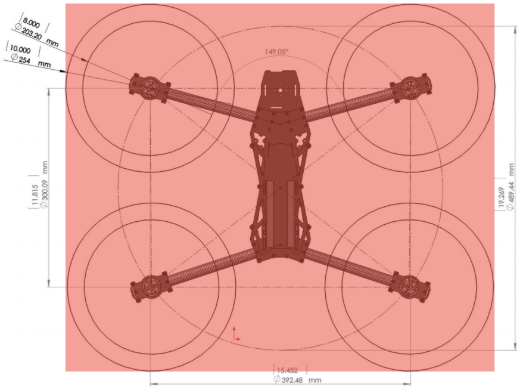
\includegraphics[width=\linewidth]{appendices/rrt/img/DroneRecPrism.png}
    \caption{}
    \label{subfig:dronerecprism}
\end{subfigure}
\end{tabular}
\caption[Modelling a UAV as a Rectangular Prism]{Modelling a \gls{UAV} as a Rectangular Prism. Red highlight demonstrates the model, overlayed over the exact schematic. Figure \ref{subfig:dronenegspace} shows how a drone can be modelled in high detail, but gains little useful free space when compared with Figure \ref{subfig:dronerecprism}, which models a drone as a rectangular prism.\cite{Thingbits}}
\label{fig:dronemodelling}
\end{centering}
\end{figure}

\section{Full Technical Specifications for RRT Implementation}
\label{section:rrt_appendix_tech_specs}
    % @Author: AnthonyKenny98
% @Date:   2020-04-05 14:09:51
% @Last Modified by:   AnthonyKenny98
% @Last Modified time: 2020-04-05 16:18:12

\begin{table}[H]
\begin{center}
\begin{tabular}{|p{.2\linewidth}|p{.74\linewidth}|}
    \hline
    \multicolumn{2}{|c|}{\textbf{General Specifications}} \\
    \hline
    \textbf{Requirement}             & \textbf{Description and Justification} \\
    \hline
    Implemented in C/C++    & 
        As outlined in Section \ref{subsection:project_structure}, the critical step in determining the design of specialized hardware to accelerate \gls{RRT} is CPU performance analysis of the algorithm to determine computational hot-spots. Implementations in C allow for the use of certain CPU profiling tools, described in Section \ref{subsubsection:vtune}, unlike higher-level languages such as Python. \\
    \hline
    3D Workspace            & 
        The computational requirements of \gls{RRT} in \gls{3D} differs somewhat to that in \gls{2D}. Since autonomous \glspl{UAV} operate in 3D space, it was neccesary to have a \gls{3D} implementation to analyse. \\
    \hline
    \Gls{UAV} modelled in \gls{3D} as a rectangular prism  & 
        In theory, it is possible to model a \gls{UAV} much more precisely than a rectangular prism, taking into account its shape and negative space. However, in reality, modelling a \gls{UAV} as a \gls{3D} rectangular prism, defined by coordinates $\{x, y, z\}$ and Euler angles $\{\alpha, \beta, \gamma \}$, is more than sufficient (and more efficient). See Appendix \ref{section:rrt_appendix_modelling} for justification of this. \\
    \hline
    Mathematically Complete Collision Detection & 
        When \gls{RRT} is implemented for educational purposes, the edge collision calulations are often simplified to a sampling model which is \gls{probabilistically complete} but not \gls{mathematically complete}. In other words, it will catch most collisions by sampling a number of points along each edge, but there is always a possibility of an undetected collision. In real world applications, collisions must be calculated by method of geometric intersection to ensure all collisions are detected. \\
    \hline
\end{tabular}
\caption{General Technical Specifications for \gls{RRT} Implementation}
\label{table:RRT_Tech_Specs_General}
\end{center}
\end{table}

\begin{table}[H]
\begin{center}
\begin{tabular}{|p{.2\linewidth}|p{.74\linewidth}|}
    \hline
    \multicolumn{2}{|c|}{\textbf{Required Parameters}} \\
    \hline
    \textbf{Parameter}   & \textbf{Description and Justification} \\
    \hline
    $\epsilon$ (a.k.a. $\Delta q$) & 
        The maximum difference between two configurations. Larger values of $\epsilon$ can solve less obstacle dense problems faster, but take longer to solve problems with tight corners.\\
    \hline
    $K$ &
        The maximum number of configurations. This is largely correlative to the amount of time the user will allow the algorithm to run. Larger values of $K$ will take longer but generate better paths, while smaller values will execute for less time but generate more jagged paths or may not reach the goal node. The value of $K$ was varied to find the minimum execution time while still reaching the goal with high probability. \\
    \hline
    $DIM$ &
        The upper bound of each axis of a $DIM\times DIM\times DIM$ Workspace. Larger values leave more space to be explored, and thus require larger values of $K$ to reach the goal with high likihood. \\
    \hline
    Goal Bias &
        The given probability that the graph will extend the graph $\epsilon$ distance from an existing configuration to a new configuration in the direction of the goal. \\
    \hline
\end{tabular}
\caption{Requiremed Parameters for \gls{RRT} Implementation}
\label{table:RRT_Tech_Specs_Parameters}
\end{center}
\end{table}

\section{Assessment of Existing RRT Implementations}
\label{section:rrt_appendix_existing_implementations}
    % @Author: AnthonyKenny98
% @Date:   2020-04-05 13:32:41
% @Last Modified by:   AnthonyKenny98
% @Last Modified time: 2020-04-05 13:46:28

\begin{table}[H]
\begin{centering}
\begin{tabular}{|p{0.2\linewidth}|p{0.15\linewidth}|p{0.15\linewidth}|p{0.15\linewidth}|p{0.15\linewidth}|}
\hline
Repository  & Language  &  Workspace Dimension  & Object Model & Algorithmic Correctness \\
\hline
RoboJackets\cite{RoboJackets2019}   & \textcolor{mygreen}{C++}    &       &       & \\
\hline
\end{tabular}
\caption[Evaluation of Existing Open-Source Implementations of RRT]{Evaluation of Existing Open-Source Implementations of RRT. Links to Github repositories can be found in the Bibliography.}
\end{centering}
\end{table}

\newpage
\section{Justification of K:DIM Ratio}